\chapter{Sklejanie grafów}

Generowanie grafów wysokiego rzędu jest bardzo wymagające zarówno czasowo jak i pamięciowo. Dlatego stosujemy technikę nazywaną sklejaniem grafów. 
\begin{definition}
Sklejanie grafów opiera się na połączeniu dwóch grafów w celu uzyskania zbioru grafów o pożądanych charakterystykach.
\end{definition}
\section{Dekompozycja problemu}
\begin{definition}
  Niech $F$ jest grafem, $v \in V(F)$, $W \subseteq V(F)$. 
  Funkcja $N_F(v,W)$ będzie zwracać podzbiór wierzchołków $W$, które sąsiadują z $v$: 
  $$N_F(v,W) = \{w \in W | (v,w) \in E(F)\}$$ 
\end{definition}

\begin{definition}
  $F[V(F) - {v}]$ będziemy zapisywać jako $F - v$.
\end{definition}

\begin{theorem}
  Niech $F$ jest grafem i $x \in V(F)$. Niech $G_x = F[N_F(x,V(F))]$
  oraz $H_x = F[V(X) - N_F(x,V(F) - x)]$. Jeśli $F$ jest $R(4,5,25)$ to 
  $G_x$ jest $R(3,5,d)$ a $F_x$ jest $R(4,4,24-d)$.
\end{theorem}

\begin{proof}

  Niech graf $F$ zawiera przynajmniej jedną klikę $K_3$ oraz przynajmniej jeden zbiór niezależny $N_4$.
  Zauważmy że dla każdej kilki $K_3$ zachodzi jedna z sytuacji:
  \begin{enumerate}
    \item $x \in K_3$
    \item $ \exists v \in K_3, (v, x) \in E(F) \land \not \forall u \in K_3, (u,x) \in E(F)$ 
    \item $\nexists v \in K_3, (v, x) \in E(F)$
  \end{enumerate} 
  
  W przypadku pierwszym klika zostanie rozbita, dwa jej wierzchołki będą w $G_x$, a $x$ nie będzie w żadnym.
  
  W przypadku drugim wierzchołki tworzące $K_3$, które są połączone z $x$ trafią do $G_x$, niepołączone trafią do $H_x$.
  
  W przypadku trzecim całość $K_3$ trafi do grafu $H_x$, gdzie klika $K_3$ może się pojawić, nie łamiąc $R(4,4,n)$.

  Z kolei dla każdego zbioru $N_4$ musi zachodzić jedna z sytuacji:

  \begin{enumerate}
    \item $x \in N_4$
    \item $ \exists v \in N_4, (v, x) \in E(F) \land \not \forall u \in N_4, (u,x) \in E(F)$ 
    \item $\nexists v \in N_4, (v, x) \in E(F)$
  \end{enumerate} 

  W przypadku pierwszym zbiór niezależny zostanie rozbity, trzy jego wierzchołki będą w $H_x$, a $x$ nie będzie w żadnym.
  
  W przypadku drugim wierzchołki tworzące $N_4$, które są połączone z $x$ trafią do $G_x$, niepołączone trafią do $H_x$.
  
  W przypadku trzecim całość $N_4$ trafi do grafu $G_x$, gdzie zbiór niezależny może się pojawić, nie łamiąc $R(3,5,n)$.
  \end{proof}

\section{Grafy potrzebne do sklejania}

Korzystając z wiedzy z poprzedniego podrozdziału możemy stwierdzić, że do utworzenia wszystkich grafów $R(4,5,24)$ wystarczy połączenie na wszystkie możliwe sposoby
wszystkich nieizomorficznych grafów $R(3,5,d)$ z wszystkimi nieizomorficznymi grafami $R(4,4,24-d)$. 
Warto zauważyć, że liczby $R(3,5)$ oraz $R(4,4)$ są znane i wynoszą odpowiednio 14 i 18. Oznacza to, że nasze grafy $G$ będą maksymalnie rzędu 13 a grafy $H$ rzędu 17. Co za tym idzie, możemy też wskazać ograniczenia dolne:
minimalny rząd $G$ to $24-17=7$ a minimalny rząd $H$ to $24-13 = 11$.  

Zbiór danych wymagany do poprawnego sklejania jest uzyskany poprzez wygenerowanie wszystkich nieizomorficznych grafów $G$ rzędów 7-13 spełniających R(3,5,$n$), oraz wszystkich nieizomorficznych grafów $H$ rzędów 11-17 spełniających R(4,4,$n$).

Grafy dzielone są na grupy zgodnie z ich rzędem. Dalsze sklejanie przeprowadzone jest na parze grup grafów $G$ i $H$. Celem sklejania jest uzyskanie grafów rzędu 24 poprzez połączenie grafów $G$ oraz $H$, a więc suma rzędów grafów $G$ oraz $H$ w grupach branych pod uwagę musi być równa 24. Oznacza to, że istnieje 6 par grup spełniających wymagania.

\section{Algorytm sklejania}

Na dalszych etapach sklejania pojawia się pojęcie stożka. Szczególnym przypadkiem stożka używanym na etapie poszukiwania połączeń grafów $G$ oraz $H$ jest stożek prawdopodobny.

\begin{definition} Stożek to podzbiór wierzchołków dowolnego grafu.
\end{definition}

\begin{definition}
Prawdopodobny stożek (ang. feasible cone) to podzbiór wierzchołków grafu H, który nie tworzy kliki $K_3$\cite{mainpaper}. Symbolizuje on połączenia pomiędzy wierzchołkiem grafu $G$ a wszystkimi wierzchołkami $V(H)$, które należą do stożka.
\end{definition}

Podzbiór wierzchołków grafu $H$ o którym jeszcze nie wiemy, czy jest prawdopodobnym stożkiem będziemy  określać mianem stożka.

Dla przeciętnego grafu R(4, 4, 14) znajdziemy około 4000 prawdopodobnych stożków. Jeżeli do każdego z wierzchołków grafu $G$ przypiszemy stożek, uzyskamy takie połączenie grafów $G$ oraz $H$ gdzie każdy wierzchołek grafu $G$ jest sąsiadem wszystkich wierzchołków w przypisanym mu stożku. Główna część algorytmu sklejania polega na eliminacji wszystkich kombinacji stożków, które prowadzą do powstania kilki rzędu 4 lub zbioru niezależnego rzędu 5. Każdy taki zbiór prawdopodobnych stożków zawiera poprawne połączenia grafów $G$ oraz $H$. Następnie zbiory prawdopodobnych stożków są rozbijane, aby wyizolować jedynie akceptowalne grafy. Taki algorytm sklejania pozwala uzyskać grafy $R(4,5,n)$ o różnych rzędach (poprzez inne parowanie grup grafów $G$ i $H$), ale w tej pracy zajmujemy się jedynie grafami 24-wierzchołkowymi.

Pierwszym etapem sklejania grafów jest stworzenie dla danego grafu $H$ zbioru prawdopodobnych stożków przed wybraniem grafu $G$ do sklejenia. Należy odrzucić wszystkie stożki które obejmują klikę stopnia trzy. Takie stożki eliminują wszystkie grafy wynikowe ponieważ połączenie kliki stopnia trzy z dowolnym wierzchołkiem powoduje wystąpienie kliki stopnia cztery. Podejście naiwne, czyli pojedyncze sprawdzenie wszystkich potencjalnie prawdopodobnych stożków nie jest jednak opłacalne ze względu na że ilość stożków dla grafu $n$ wierzchołkowego, która jest równa $2^n$. W celu przyspieszenia obliczeń stożki grupowane są w przedziały. 

\begin{definition}
Przedział $P = [B, T]$ to zbiór stożków, ograniczony przez stożek górny $T_P$ i stożek dolny $B_P$, który zawiera wszystkie stożki spełniające zależność:  $$P=\{X: B_P \subseteq X \subseteq T_P\}$$ 
\end{definition}


Znajdowanie prawdopodobnych stożków rozpoczynamy od pojedynczego przedziału gdzie $B_P = \emptyset$, a $T_P$ zawiera wszystkie wierzchołki $H$. Taki przedział zawiera wszystkie możliwe stożki. W celu wyodrębnienia prawdopodobnych stożków korzystamy z poniższych własności:
\begin{enumerate}
\item Dla wierzchołka $w$, który spełnia $w \notin B_P$ oraz $w\in T_P$ prawdą jest, że $[B_P, T_P] = [B_P \cup \{ w\}, T_P] \cup [B_P , T_P \setminus \{ w\}]$ oraz $[B_P +\{ w\}, T_P] \cap [B_P , T_P - \{ w\}] = \emptyset$. 

\item Jeżeli $H[B_P]$ zawiera klikę stopnia 3, to wszystkie stożki w przedziale również ją zawierają. 

\item Jeżeli $H[T_P]$ nie zawiera kliki stopnia 3, to wszystkie stożki w przedziale jej nie zawierają.
\end{enumerate}

Korzystając z własności 2 i 3 jako warunku odpowiednio odrzucenia lub zaakceptowania przedziału można skorzystać z algorytmu rekurencyjnego dzielącego interwały wzdłuż wierzchołków należących do kliki 3 oraz stożka $B$, dzięki czemu uzyskujemy zbiór przedziałów dla grafu $H$ zawierający jedynie stożki prawdopodobne. Z tego zbioru korzystamy w następnym etapie algorytmu.
Dalsze odrzucanie stożków musi odbyć się już w kontekście grafu $G$.
  

\section{Zawężanie przedziałów - zasady A-D}
Zdefiniujmy 3 funkcje pomocnicze działające na podzbiorze wierzchołków grafu $H$ oznaczonym jako $X$, generujące podzbiór wierzchołków grafu $H$. 
Funkcja $H_1$ będzie wybierała wszystkich sąsiadów wierzchołków ze zbioru $X$.
$H_2$ wybiera wszystkie wierzchołki, które nie sąsiadują z jednym lub większą ilością wierzchołków spoza $X$. 
$H_3$ wybiera wszystkie wierzchołki, które tworzą zbiór niezależny o stopniu 3 z dwoma wierzchołkami spoza zbioru $X$.

$$H_i: P(x) \to P(x)$$

\begin{itemize}
    
  \item   $H_1(X) = \{ w \in V(H) | vw \in E(X) \textrm{ dla jakiegoś } v \in X \}$ 
  
  \item   $H_2(X) = \{ w \in V(H) | vw \notin E(X) \textrm{ dla jakiegoś } v \notin X\}$
  
  \item   $H_3(X) = \{ w \in V(H) | { u, v, w } \textrm{ jest zbiorem niezależnym dla jakichś } v, u \notin X\}$ 
\end{itemize}


Rozpatrzmy graf na rysunku \ref{zasada0}. Dla tego grafu zostanie zaprezentowanie działanie zasad  $H_1$,  $H_2$ oraz  $H_3$. Na rysunkach \ref{zasada1}, \ref{zasada2}, \ref{zasada3}, przedstawiony jest sposób działania tych funkcji. Pierwszy graf jest grafem, który jest przekazywany do funkcji, a wierzchołki zaznaczone na niebiesko oznaczają wierzchołki ze zbioru $X$. Drugi graf zawiera wierzchołki zaznaczone na czerwono, jest to podzbiór wierzchołków które zwraca funkcja.


 \begin{figure}[H]
  \centering
   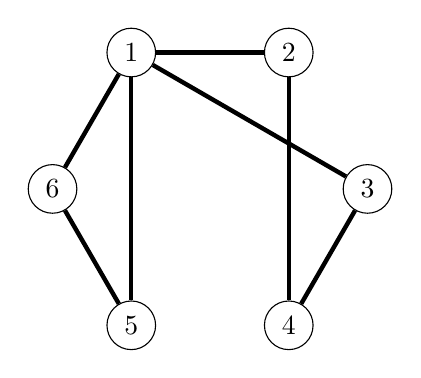
\begin{tikzpicture}[node distance={15mm}, main/.style = {draw, circle}] 
 \node[main] (3) at (0:2) {$3$};
 \node[main] (2) at (60:2) {$2$};
 \node[main] (1) at (120:2) {$1$};
 \node[main] (6) at (180:2) {$6$};
 \node[main] (5) at (240:2) {$5$};
 \node[main] (4) at (300:2) {$4$};

\draw[ultra thick] (1) -- (2);
\draw[ultra thick] (1) -- (3);
\draw[ultra thick] (1) -- (6);
\draw[ultra thick] (1) -- (5);
\draw[ultra thick] (6) -- (5);
\draw[ultra thick] (2) -- (4);
\draw[ultra thick] (3) -- (4);
    \end{tikzpicture}
    \caption{Graf służący do zaprezentowania poszczególnych funkcji $H$}
 \label{zasada0}
 \end{figure}

Funkcja $H_1$ znajduje wszystkich sąsiadów wierzchołków ze zbioru wejściowego. W podanym przykładzie na rysunku \ref{zasada1} oznacza to, że musimy znaleźć sąsiadów wierzchołków ze zbioru \{3, 4\}. Łatwo zauważyć że wierzchołki z nimi sąsiadujące to zbiór wierzchołków \{1, 2, 3, 4\}.

 \begin{figure}[H]
  \centering
  \subfloat[]{
   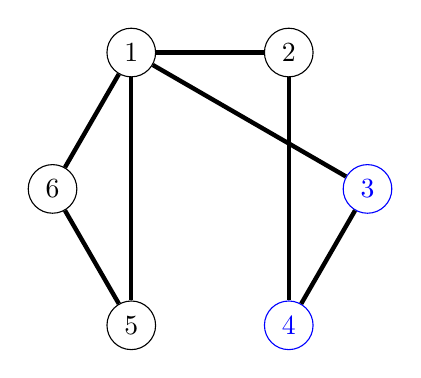
\begin{tikzpicture}[node distance={15mm}, main/.style = {draw, circle}] 
 \node[main][blue]  (3) at (0:2) {$3$};
 \node[main] (2) at (60:2) {$2$};
 \node[main] (1) at (120:2) {$1$};
 \node[main] (6) at (180:2) {$6$};
 \node[main] (5) at (240:2) {$5$};
 \node[main][blue]  (4) at (300:2) {$4$};

\draw[ultra thick] (1) -- (2);
\draw[ultra thick] (1) -- (3);
\draw[ultra thick] (1) -- (6);
\draw[ultra thick] (1) -- (5);
\draw[ultra thick] (6) -- (5);
\draw[ultra thick] (2) -- (4);
\draw[ultra thick] (3) -- (4);
    \end{tikzpicture}
    }
    \hspace{15mm}
    \subfloat[]{
   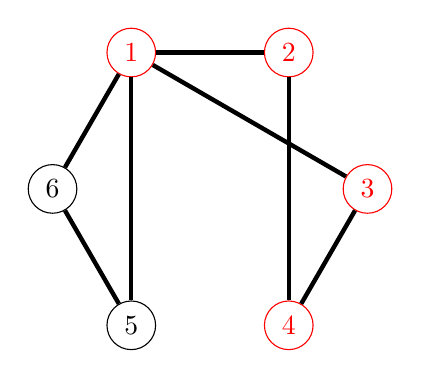
\begin{tikzpicture}[node distance={15mm}, main/.style = {draw, circle}] 
 \node[main][red] (3) at (0:2) {$3$};
 \node[main][red] (2) at (60:2) {$2$};
 \node[main][red] (1) at (120:2) {$1$};
 \node[main] (6) at (180:2) {$6$};
 \node[main] (5) at (240:2) {$5$};
 \node[main][red] (4) at (300:2) {$4$};

\draw[ultra thick] (1) -- (2);
\draw[ultra thick] (1) -- (3);
\draw[ultra thick] (1) -- (6);
\draw[ultra thick] (1) -- (5);
\draw[ultra thick] (6) -- (5);
\draw[ultra thick] (2) -- (4);
\draw[ultra thick] (3) -- (4);
    \end{tikzpicture}
    }
    \caption{Wynik działania funkcji $H_1$}
 \label{zasada1}
 \end{figure}

Funkcja $H_2$ znajduje wszystkie wierzchołki, które nie sąsiadują z co najmniej jednym wierzchołkiem spoza zbioru wejściowego. W podanym przykładzie na rysunku \ref{zasada2} oznacza to że musimy znaleźć wierzchołki które nie sąsiadują ze wszystkimi wierzchołkami ze zbioru (wykluczając wierzchołek który aktualnie rozpatrujemy, jeżeli jest w zbiorze) \{1, 2, 5, 6\}. Łatwo zauważyć że jedynym wierzchołkiem który sąsiaduje ze wszystkimi wierzchołkami z tego zbioru jest wierzchołek o numerze 1, więc zbiór wyjściowy będzie wyglądać następująco \{2, 3, 4, 5, 6\}.

 \begin{figure}[H]
  \centering
  \subfloat[]{
   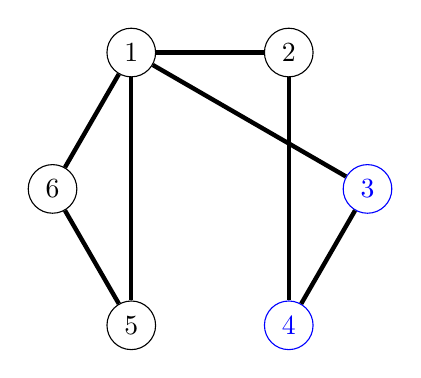
\begin{tikzpicture}[node distance={15mm}, main/.style = {draw, circle}] 
 \node[main][blue]  (3) at (0:2) {$3$};
 \node[main] (2) at (60:2) {$2$};
 \node[main] (1) at (120:2) {$1$};
 \node[main] (6) at (180:2) {$6$};
 \node[main] (5) at (240:2) {$5$};
 \node[main][blue]  (4) at (300:2) {$4$};

\draw[ultra thick] (1) -- (2);
\draw[ultra thick] (1) -- (3);
\draw[ultra thick] (1) -- (6);
\draw[ultra thick] (1) -- (5);
\draw[ultra thick] (6) -- (5);
\draw[ultra thick] (2) -- (4);
\draw[ultra thick] (3) -- (4);
    \end{tikzpicture}
    }
    \hspace{15mm}
    \subfloat[]{
   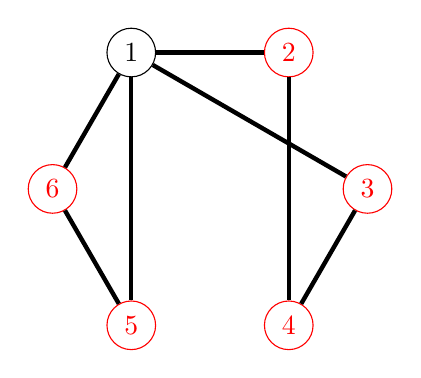
\begin{tikzpicture}[node distance={15mm}, main/.style = {draw, circle}] 
 \node[main][red] (3) at (0:2) {$3$};
 \node[main][red] (2) at (60:2) {$2$};
 \node[main] (1) at (120:2) {$1$};
 \node[main][red] (6) at (180:2) {$6$};
 \node[main][red] (5) at (240:2) {$5$};
 \node[main][red] (4) at (300:2) {$4$};

\draw[ultra thick] (1) -- (2);
\draw[ultra thick] (1) -- (3);
\draw[ultra thick] (1) -- (6);
\draw[ultra thick] (1) -- (5);
\draw[ultra thick] (6) -- (5);
\draw[ultra thick] (2) -- (4);
\draw[ultra thick] (3) -- (4);
    \end{tikzpicture}
    }
    \caption{Wynik działania funkcji $H_2$}
 \label{zasada2}
 \end{figure}

Funkcja $H_3$ znajduje wszystkie wierzchołki, które tworzą zbiór niezależny o stopniu 3 z dwoma wierzchołkami spoza zbioru $X$. W podanym przykładzie na rysunku \ref{zasada3} oznacza to, że musimy znaleźć wierzchołki które tworzą zbiór niezależny wraz z dwoma wierzchołkami ze zbioru \{1, 2, 5, 6\}. Łatwo zauważyć że jedynym wierzchołkiem który spełnia to założenie jest wierzchołek oznaczony numerem 3, gdyż tworzy on zbiór niezależny stopnia 3 wraz z wierzchołkami o numerach 2 oraz 5.

 \begin{figure}[H]
  \centering
  \subfloat[]{
   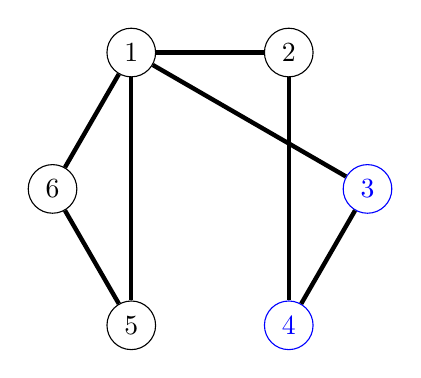
\begin{tikzpicture}[node distance={15mm}, main/.style = {draw, circle}] 
 \node[main][blue]  (3) at (0:2) {$3$};
 \node[main] (2) at (60:2) {$2$};
 \node[main] (1) at (120:2) {$1$};
 \node[main] (6) at (180:2) {$6$};
 \node[main] (5) at (240:2) {$5$};
 \node[main][blue]  (4) at (300:2) {$4$};

\draw[ultra thick] (1) -- (2);
\draw[ultra thick] (1) -- (3);
\draw[ultra thick] (1) -- (6);
\draw[ultra thick] (1) -- (5);
\draw[ultra thick] (6) -- (5);
\draw[ultra thick] (2) -- (4);
\draw[ultra thick] (3) -- (4);
    \end{tikzpicture}
    }
    \hspace{15mm}
    \subfloat[]{
   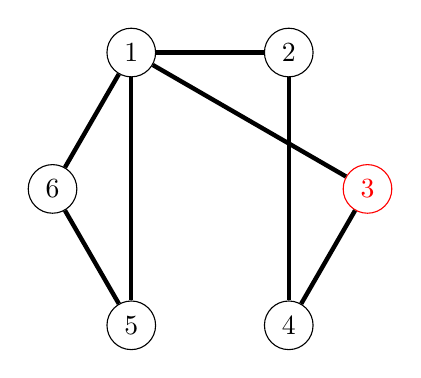
\begin{tikzpicture}[node distance={15mm}, main/.style = {draw, circle}] 
 \node[main][red] (3) at (0:2) {$3$};
 \node[main] (2) at (60:2) {$2$};
 \node[main] (1) at (120:2) {$1$};
 \node[main] (6) at (180:2) {$6$};
 \node[main] (5) at (240:2) {$5$};
 \node[main] (4) at (300:2) {$4$};

\draw[ultra thick] (1) -- (2);
\draw[ultra thick] (1) -- (3);
\draw[ultra thick] (1) -- (6);
\draw[ultra thick] (1) -- (5);
\draw[ultra thick] (6) -- (5);
\draw[ultra thick] (2) -- (4);
\draw[ultra thick] (3) -- (4);
    \end{tikzpicture}
    }
    \caption{Wynik działania funkcji $H_3$}
 \label{zasada3}
 \end{figure}


Kolejny etap zawężania zbioru potencjalnych krawędzi pomiędzy grafami $G$ oraz $H$ odbywa się już w kontekście konkretnego grafu $G$. Każda możliwa kombinacja wygenerowanych przedziałów jest  przydzielana do wierzchołków należących do $G$, dzięki czemu rozważone są wszystkie możliwe sposoby połączenia tych grafów. Dla każdego zbioru przedziałów łączących grafy $G$ oraz $H$ wykonywany jest poniższy zbiór reguł działających na wierzchołki i przedziały stożków im przypisane:
\begin{itemize}
  \item[A] - stosowana do 2 wierzchołków $u,v$ $\in G$ sąsiadujących ze sobą 
  
  Jeśli $B_u \cap B_v \cap H_1(B_u \cap B_v) \neq \emptyset $ to nie da się 
  poprawnie skleić tej pary grafów przy użyciu tej permutacji przedziałów.
  
  W innym wypadku z $T_u$ usuwamy $H_1(B_u \cap B_v) \cap B_v $  
  \item[B] - stosowana do 2 wierzchołków $u,v$ $\in G$ nie sąsiadujących ze sobą 
  
  Jeśli $H_3(T_u \cup T_v) \not\subseteq (T_u \cup T_v)$ to nie da się poprawnie skleić tej pary grafów przy użyciu tej permutacji przedziałów.
  
  W innym wypadku $B_u$ rozszerzamy do $B_u \cup (H_3(T_u \cup T_v) - T_v)$
  \item[C] - stosowana do 3 wierzchołków $u,v,w$ $\in G$ tworzących zbiór niezależny $N_3$ 
  
  Jeśli $H_2(T_u \cup T_v \cup T_w) \not\subseteq (T_u \cup T_v \cup T_w)$ 
  to nie da się poprawnie skleić tej pary grafów przy użyciu tej permutacji przedziałów. 
  
  W innym wypadku $B_u$ rozszerzamy do $B_u \cup (H_2(T_u \cup T_v \cup T_w) - (T_v \cup T_w))$
  \item[D] - stosowana do 4 wierzchołków $u,v,w,z$ $\in G$ tworzących zbiór niezależny $N_4$  
  
  Jeśli $T_u \cup T_v \cup T_w \cup \neq V(H) $ to nie da się poprawnie skleić tej pary grafów przy użyciu tej permutacji przedziałów.
  
  W innym wypadku $B_u$ rozszerzamy do $B_u \cup (VH - (T_v \cup T_w \cup T_z))$
\end{itemize}

Zasada A sprawdza czy sąsiednie wierzchołki $u, v$ mają jakąkolwiek parę wspólnych potencjalnych sąsiadów, którzy są sąsiedni względem siebie.
W takiej sytuacji powstałaby klika $K_4$, więc nie uda się utworzyć grafu. \par

Przyjrzyjmy się rysunkowi \ref{zasadaA1}. Czerwone wierzchołki to $u, v$ z grafu $G$, 
a czerwone, przerywane krawędzie reprezentują dolne ograniczenia przypisanych im stożków.
Jak widać, $u$ i $v$ muszą zostać połączone z parą sąsiadujących wierzchołków 1 i 2, więc nie 
da się poprawnie połączyć grafów użyciem takiego przypisania stożków.
\begin{figure}[H]
  \centering
   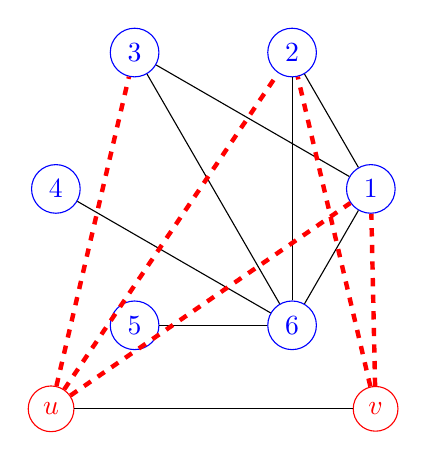
\begin{tikzpicture}[node distance={15mm}, main/.style = {draw, circle}] 
    
    \node[main][blue] (1) at (0:2) {$1$};
    \node[main][blue] (2) at (60:2) {$2$};
    \node[main][blue] (3) at (120:2) {$3$};
    \node[main][blue] (4) at (180:2) {$4$};
    \node[main][blue] (5) at (240:2) {$5$};
    \node[main][blue] (6) at (300:2) {$6$};

    \draw (1) -- (2);
    \draw (1) -- (3);
    \draw (6) -- (1);
    \draw (6) -- (2);
    \draw (6) -- (3);
    \draw (6) -- (4);
    \draw (6) -- (5);

    \vspace{10mm};

    \node[main][red] (7) [below left of=5] {$u$};
    \node[main][red] (8) [below right of=6] {$v$};

    \draw (7) -- (8);

    \draw [ultra thick][red, dashed] (7) -- (3);
    \draw [ultra thick][red, dashed] (7) -- (1);
    \draw [ultra thick][red, dashed] (7) -- (2);

    \draw [ultra thick][red, dashed] (8) -- (1);
    \draw [ultra thick][red, dashed] (8) -- (2);

\end{tikzpicture}
 \caption{Przykład sytuacji odrzucanej przez zasadę A}
 \label{zasadaA1}
 \end{figure}

 Jeżeli powyższa sytuacja nie zajdzie, musimy usunąć z $T_u$ niezbędnych sąsiadów $v$, 
 którzy sąsiadują z przynajmniej jednym z niezbędnych sąsiadów $u$. 
 
  Na rysunku \ref{zasadaA2} wprowadzono ograniczenie górne, reprezentowane niebieskimi, 
  przerywanymi krawędziami.  Jak widać, to połączenie nie jest odrzucane (istnieje możliwość połączenie bez utworzenia $K_4$).
    
  Trzeba więc odrzucić potencjalne połączenia pomiędzy $v$ a niezbędnymi sąsiadami $u$. 
  Na przykładowym rysunku będzie to oznaczało usunięcie krawędzi $(u, 5)$. Zgodnie z zasadą A nie usuwamy jeszcze krawędzi 
  $(v,2)$ - zostanie ona usunięta kiedy to $v$ będzie pełniła rolę $u$ w funkcji.  

 \begin{figure}[H]
  \centering
   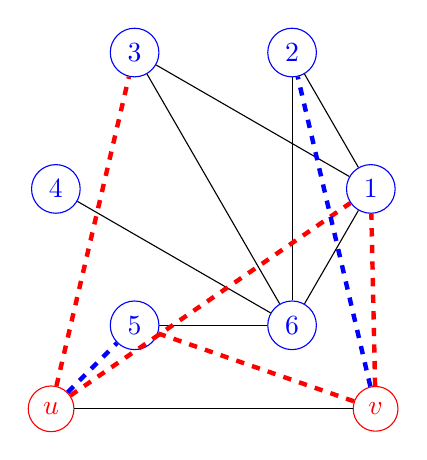
\begin{tikzpicture}[node distance={15mm}, main/.style = {draw, circle}] 
    
    \node[main][blue] (1) at (0:2) {$1$};
    \node[main][blue] (2) at (60:2) {$2$};
    \node[main][blue] (3) at (120:2) {$3$};
    \node[main][blue] (4) at (180:2) {$4$};
    \node[main][blue] (5) at (240:2) {$5$};
    \node[main][blue] (6) at (300:2) {$6$};

    \draw (1) -- (2);
    \draw (1) -- (3);
    \draw (6) -- (1);
    \draw (6) -- (2);
    \draw (6) -- (3);
    \draw (6) -- (4);
    \draw (6) -- (5);

    \vspace{20mm};

    \node[main][red] (7) [below left of=5] {$u$};
    \node[main][red] (8) [below right of=6] {$v$};

    \draw (7) -- (8);

    \draw [ultra thick][red, dashed] (7) -- (3);
    \draw [ultra thick][red, dashed] (7) -- (1);
    \draw [ultra thick][blue, dashed] (7) -- (5);

    \draw [ultra thick][red, dashed] (8) -- (1);
    \draw [ultra thick][red, dashed] (8) -- (5);
    \draw [ultra thick][blue, dashed] (8) -- (2);

\end{tikzpicture}
 \caption{Przykład przedziału zawężanego przez zasadę A}
 \label{zasadaA2}
 \end{figure}

Zasada B sprawdza czy istnieją w grafie $H$ zbiory niezależne $N_3$, z których wierzchołkami żaden z wierzchołków $u, v$ nie może zostać połączony. W takim wypadku nie da się skleić grafów bez utworzenia zbioru niezależnego $N_5$. 

Dla przykładu, przeanalizujmy rysunek \ref{zasadaB1}. Wierzchołki 2, 4, 6 tworzą zbiór niezależny i żaden z nich nie mieści się w ograniczeniach głównych wierzchołków 
$u, v$. W związku z tym, dana próba połączenia nie zakończy się sukcesem. 

\begin{figure}[H]
  \centering
   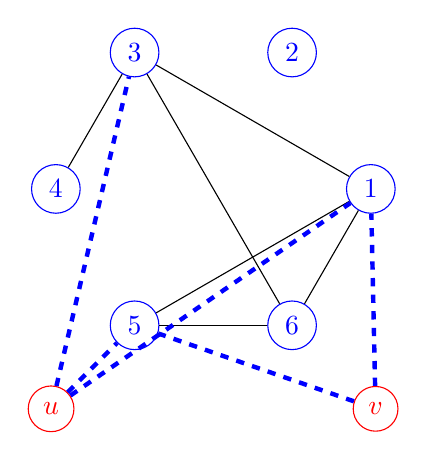
\begin{tikzpicture}[node distance={15mm}, main/.style = {draw, circle}] 
    
    \node[main][blue] (1) at (0:2) {$1$};
    \node[main][blue] (2) at (60:2) {$2$};
    \node[main][blue] (3) at (120:2) {$3$};
    \node[main][blue] (4) at (180:2) {$4$};
    \node[main][blue] (5) at (240:2) {$5$};
    \node[main][blue] (6) at (300:2) {$6$};

    \draw (3) -- (1);
    \draw (6) -- (1);
    \draw (6) -- (3);
    \draw (6) -- (5);
    \draw (5) -- (1);
    \draw (4) -- (3);

    \vspace{20mm};

    \node[main][red] (7) [below left of=5] {$u$};
    \node[main][red] (8) [below right of=6] {$v$};

    \draw [ultra thick][blue, dashed] (7) -- (3);
    \draw [ultra thick][blue, dashed] (7) -- (1);
    \draw [ultra thick][blue, dashed] (7) -- (5);

    \draw [ultra thick][blue, dashed] (8) -- (1);
    \draw [ultra thick][blue, dashed] (8) -- (5);

\end{tikzpicture}
 \caption{Przykład sytuacji odrzucanej przez zasadę B}
 \label{zasadaB1}
 \end{figure}

Jeżeli powyższa sytuacja nie zachodzi, musimy do zbioru $B_u$ dodać wszystkie wierzchołki, 
z którymi przynajmniej 2 wierzchołki spoza zbioru $T_u \cup T_v$ nie sąsiadują. Wyjątkiem są te, z którymi można połączyć $v$. \par

W przykładzie z rysunku \ref{zasadaB2} trzeba dodać wierzchołek 4 do dolnego ograniczenia $u$.
\begin{figure}[H]
  \centering
   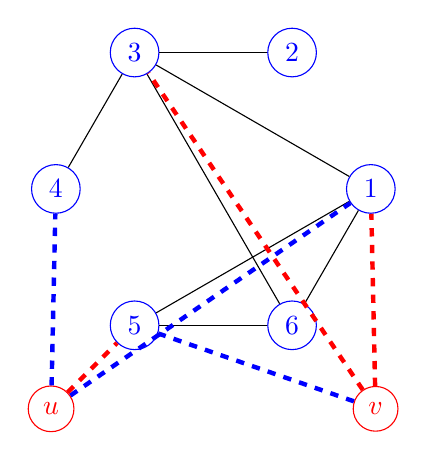
\begin{tikzpicture}[node distance={15mm}, main/.style = {draw, circle}] 
    
    \node[main][blue] (1) at (0:2) {$1$};
    \node[main][blue] (2) at (60:2) {$2$};
    \node[main][blue] (3) at (120:2) {$3$};
    \node[main][blue] (4) at (180:2) {$4$};
    \node[main][blue] (5) at (240:2) {$5$};
    \node[main][blue] (6) at (300:2) {$6$};

    \draw (3) -- (1);
    \draw (6) -- (1);
    \draw (6) -- (3);
    \draw (6) -- (5);
    \draw (5) -- (1);
    \draw (4) -- (3);
    \draw (2) -- (3);

    \vspace{20mm};

    \node[main][red] (7) [below left of=5] {$u$};
    \node[main][red] (8) [below right of=6] {$v$};

    \draw [ultra thick][red, dashed] (8) -- (3);
    \draw [ultra thick][red, dashed] (8) -- (1);
    \draw [ultra thick][blue, dashed] (8) -- (5);

    \draw [ultra thick][blue, dashed] (7) -- (1);
    \draw [ultra thick][blue, dashed] (7) -- (4);
    \draw [ultra thick][red, dashed] (7) -- (5);

\end{tikzpicture}
 \caption{Przykład przedziału zawężanego przez zasadę B}
 \label{zasadaB2}
 \end{figure}

Zasada C sprawdza czy istnieją w grafie $H$ dwa niesąsiadujące wierzchołki, z którymi żaden z wierzchołków zbioru niezależnego $u, v, w$ nie może zostać połączony. 
Oznaczałoby to, że musi powstać zbiór niezależny $N_5$, a grafów nie można skleić.

W przykładzie z rysunku \ref{zasadaC1} musi powstać zbiór niezależny $N_5$, ponieważ żaden z wierzchołków $u, v, w$ nie może zostać połączony z którymś z niesąsiadujących 
wierzchołków 2, 4. Ten sposób połączenia zostanie więc odrzucony. 

\begin{figure}[H]
  \centering
   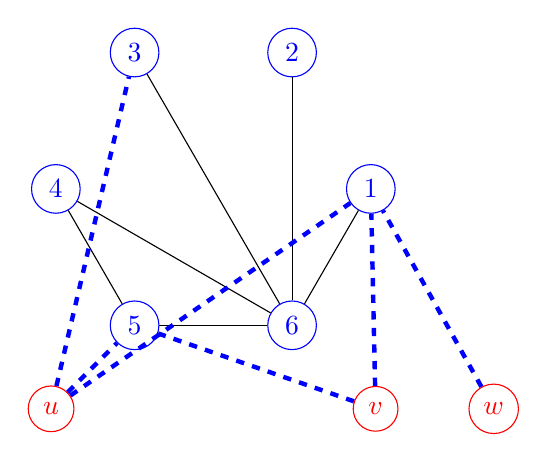
\begin{tikzpicture}[node distance={15mm}, main/.style = {draw, circle}] 
    
    \node[main][blue] (1) at (0:2) {$1$};
    \node[main][blue] (2) at (60:2) {$2$};
    \node[main][blue] (3) at (120:2) {$3$};
    \node[main][blue] (4) at (180:2) {$4$};
    \node[main][blue] (5) at (240:2) {$5$};
    \node[main][blue] (6) at (300:2) {$6$};

    \draw (6) -- (1);
    \draw (6) -- (2);
    \draw (6) -- (3);
    \draw (6) -- (4);
    \draw (6) -- (5);
    \draw (4) -- (5);

    \vspace{20mm};

    \node[main][red] (7) [below left of=5] {$u$};
    \node[main][red] (8) [below right of=6] {$v$};
    \node[main][red] (9) [right of=8] {$w$};

    \draw [ultra thick][blue, dashed] (7) -- (3);
    \draw [ultra thick][blue, dashed] (7) -- (1);
    \draw [ultra thick][blue, dashed] (7) -- (5);

    \draw [ultra thick][blue, dashed] (8) -- (1);
    \draw [ultra thick][blue, dashed] (8) -- (5);

    \draw [ultra thick][blue, dashed] (9) -- (1);

\end{tikzpicture}
 \caption{Przykład sytuacji odrzucanej przez zasadę C}
 \label{zasadaC1}
 \end{figure}

W innym wypadku do $B_u$ trzeba dodać wierzchołki które nie sąsiadują z wierzchołkiem, 
z którym żaden z wierzchołków $u, v, w$ nie może zostać połączony, z wyjątkiem tych z którymi może sąsiadować $v$ lub $w$.  \par

Dla sytuacji z rysunku \ref{zasadaC2} konieczne jest dodanie do dolnego ograniczenia dla $u$ wierzchołka 4. 
\begin{figure}[H]
  \centering
   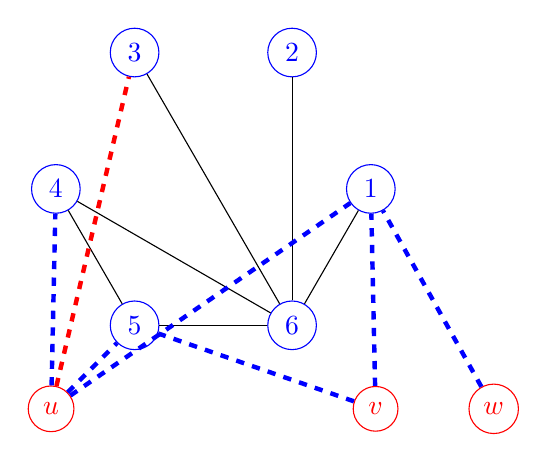
\begin{tikzpicture}[node distance={15mm}, main/.style = {draw, circle}] 
    
    \node[main][blue] (1) at (0:2) {$1$};
    \node[main][blue] (2) at (60:2) {$2$};
    \node[main][blue] (3) at (120:2) {$3$};
    \node[main][blue] (4) at (180:2) {$4$};
    \node[main][blue] (5) at (240:2) {$5$};
    \node[main][blue] (6) at (300:2) {$6$};

    \draw (6) -- (1);
    \draw (6) -- (2);
    \draw (6) -- (3);
    \draw (6) -- (4);
    \draw (6) -- (5);
    \draw (4) -- (5);

    \vspace{20mm};

    \node[main][red] (7) [below left of=5] {$u$};
    \node[main][red] (8) [below right of=6] {$v$};
    \node[main][red] (9) [right of=8] {$w$};

    \draw [ultra thick][red, dashed] (7) -- (3);
    \draw [ultra thick][blue, dashed] (7) -- (1);
    \draw [ultra thick][blue, dashed] (7) -- (5);
    \draw [ultra thick][blue, dashed] (7) -- (4);

    \draw [ultra thick][blue, dashed] (8) -- (1);
    \draw [ultra thick][blue, dashed] (8) -- (5);

    \draw [ultra thick][blue, dashed] (9) -- (1);

\end{tikzpicture}
 \caption{Przykład przedziału zawężanego przez zasadę C}
 \label{zasadaC2}
 \end{figure}

Zasada D sprawdza czy graf $H$ zawiera wierzchołek, z którym żaden z niesąsiadujących wierzchołków $u, v, w, z$
nie może sąsiadować. Ponownie, w takim przypadku powstałby zbiór niezależny $N_5$.

Na rysunku \ref{zasadaD1} żaden z wierzchołków $v, z, w, u$ nie może zostać połączony z wierzchołkiem 6. Ten sposób połączenia należy odrzucić. 
\begin{figure}[H]
  \centering
   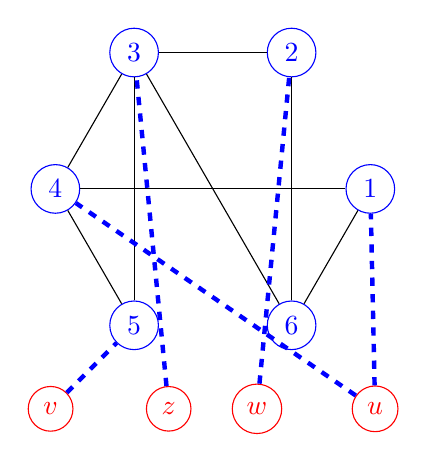
\begin{tikzpicture}[node distance={15mm}, main/.style = {draw, circle}] 
    
    \node[main][blue] (1) at (0:2) {$1$};
    \node[main][blue] (2) at (60:2) {$2$};
    \node[main][blue] (3) at (120:2) {$3$};
    \node[main][blue] (4) at (180:2) {$4$};
    \node[main][blue] (5) at (240:2) {$5$};
    \node[main][blue] (6) at (300:2) {$6$};

    \draw (6) -- (1);
    \draw (6) -- (2);
    \draw (6) -- (3);
    \draw (3) -- (4);
    \draw (4) -- (5);
    \draw (5) -- (3);
    \draw (3) -- (2);
    \draw (4) -- (1);

    \vspace{20mm};

    
    \node[main][red] (8) [below right of=6] {$u$};
    \node[main][red] (9) [below left of=5] {$v$};
    \node[main][red] (7) [left of=8] {$w$};
    \node[main][red] (10) [right of=9] {$z$};

    \draw [ultra thick][blue, dashed] (7) -- (2);
    \draw [ultra thick][blue, dashed] (8) -- (4);
    \draw [ultra thick][blue, dashed] (9) -- (5);
    \draw [ultra thick][blue, dashed] (10) -- (3);
    \draw [ultra thick][blue, dashed] (8) -- (1);
  

\end{tikzpicture}
 \caption{Przykład sytuacji odrzucanej przez zasadę D}
 \label{zasadaD1}
 \end{figure}

Jeżeli powyższe nie zajdzie, musimy dodać do $B_u$ wszystkie wierzchołki, z którymi $v, w, z$ nie mogą sąsiadować. \par

Przykładowo, na rysunku \ref{zasadaD2} $u$ jest połączone ze wszystkimi wierzchołkami 1-5, ale 1 i 2 mogą też zostać połączone z innymi wierzchołkami, więc do
$B_u$ zostanie dodany tylko wierzchołek 3.   
\begin{figure}[H]
  \centering
   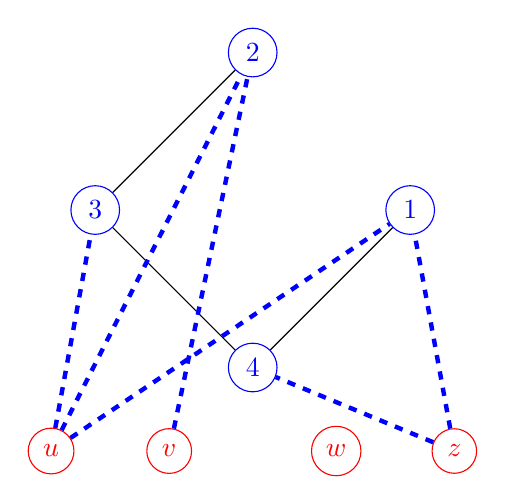
\begin{tikzpicture}[node distance={15mm}, main/.style = {draw, circle}] 
    
    \node[main][blue] (1) at (0:2) {$1$};
    \node[main][blue] (2) at (90:2) {$2$};
    \node[main][blue] (3) at (180:2) {$3$};
    \node[main][blue] (4) at (270:2) {$4$};


    \draw (3) -- (4);
    \draw (3) -- (2);
    \draw (4) -- (1);

    \vspace{20mm};

    
    \node[main][red] (8) [below right of=4] {$w$};
    \node[main][red] (9) [below left of=4] {$v$};
    \node[main][red] (7) [left of=9] {$u$};
    \node[main][red] (10) [right of=8] {$z$};

    \draw [ultra thick][blue, dashed] (7) -- (3);
    \draw [ultra thick][blue, dashed] (7) -- (2);
    \draw [ultra thick][blue, dashed] (7) -- (1);
    \draw [ultra thick][blue, dashed] (9) -- (2);
    \draw [ultra thick][blue, dashed] (10) -- (1);
    \draw [ultra thick][blue, dashed] (10) -- (4);

  

\end{tikzpicture}
 \caption{Przykład przedziału zawężanego przez zasadę D}
 \label{zasadaD2}
 \end{figure}

Warto zauważyć, że wynikiem zastosowania dowolnej reguły jest zawsze odrzucenie zestawu przedziałów, zawężenie przedziału lub brak zmian. Reguły są więc aplikowane do momentu, w którym ponowne zaaplikowanie dowolnej reguły dla dowolnych wierzchołków grafu $G$ i odpowiadających im przedziałom nie powoduje już dalszych zmian. Wynikowy zbiór przedziałów daje sposób lub sposoby połączenia grafów $G$ oraz $H$ w graf 24 wierzchołkowy spełniający wymagania pod względem ramseyowskości. Nie wszystkie sposoby połączenia pozostałe przy zatrzymaniu reguł muszą być jednak poprawne. Istnieje możliwość, że wynikowe przedziały posiadają również połączenia niepoprawne. Z tego powodu, po zakończeniu stosowania reguł należy rozbijać wynikowe przedziały, i ponownie stosować reguły, aż wynikiem ich stosowania będzie tylko jeden poprawny graf.

Przez rozbicie zestawu przedziałów mamy na myśli operację, gdzie przedział jest zamieniany na dwa przedziały przy użyciu własności przedziału numer 1. Należy rozbijać tylko te przedziały, dla których $B \neq T$, ponieważ takie przedziały obejmują więcej niż jeden stożek prawdopodobny, a więc i więcej niż jeden sposób połączenia $G$ i $H$.

\section{Rozszerzenie grafu R(4,5,24) do R(4,5,25)}

Po zakończeniu głównej części procesu sklejania uzyskujemy zbiór grafów $\mathcal{F} = R(4,5,24)$. W dalszej części pracy graf z tego zbioru będzie oznaczany jako graf $F$. Jeżeli zbiór $R(4,5,25) \neq \emptyset$ to w wyniku rozszerzenia grafów $\mathcal{F}$ powinniśmy uzyskać przynajmniej jeden graf 25 wierzchołkowy spełniający wymagania. 
Rozszerzanie zostaje w tym wypadku wykonane metodą inną od wcześniejszego generowania grafów

Metoda rozszerzania do grafu 25-wierzchołkowego jest podobna wcześniej opisanemu algorytmowi tworzenia przedziałów stożków. Największą róznicą jest to, że w tym wypadku mamy tylko jeden wierzchołek, do którego przypisywane są stożki rozszerzające.
\begin{definition}
  Stożek rozszerzający to podzbiór wierzchołków grafu $F$ symbolizujący możliwe połączenia pomiędzy grafem $F$ a wierzchołkiem do niego dodawanym.
\end{definition}

Po raz kolejny, wszystkie możliwe stożki rozszerzające są grupowane w przedział, który w trakcie działania algorytmu jest zawężany. Przedziały stożków rozszerzających mają te same własności, co przedziały stożków prawdopodobnych, w tym wypadku mają jednak znaczenie dwie dodatkowe własności:

\begin{enumerate}

\item Dla wierzchołka $w$, który spełnia $w \notin B$ oraz $w\in T$ prawdą jest, że $[B, T] = [B + \{ w\}, T] \cup [B , T - \{ w\}]$ oraz $[B +\{ w\}, T] \cap [B , T - \{ w\}] = \emptyset$

\item Jeżeli ograniczenie przedziału $B$ zawiera klikę stopnia 3, to wszystkie stożki w przedziale również ją zawierają. 

\item Jeżeli ograniczenie przedziału $T$ nie zawiera kliki stopnia 3, to wszystkie stożki w przedziale jej nie zawierają.

																													  
				 
\item Jeżeli ograniczenie przedziału $B$ zawiera przynajmniej jeden wierzchołek ze zbioru niezależnego stopnia 4, to wszystkie stożki w przedziale również go zawierają. 

\item Jeżeli ograniczenie przedziału $T$ nie zawiera żadnego wierzchołka ze zbioru niezależnego stopnia 4, wszystkie stożki w przedziale ich nie zawierają. 

\end {enumerate}

Własność pierwsza jest używana podczas opisanego później podziału przedziałów, natomiast własności 2-4 są używane jako sposób na zaakceptowanie lub odrzucenie przedziału.
Etapem przygotowawczym do rozszerzania jest stworzenie listy podzbiorów wierzchołków $F$ które tworzą kliki lub zbiory niezależne. Takie podzbiory nazywamy dalej zbiorami niedozwolonymi. 

\begin{definition} Zbiór niedozwolony to podzbiór wierzchołków grafu $F$ który nakłada ograniczenia na sposoby rozszerzenia go o wierzchołek.
\end{definition}

W przypadku rozszerzania do R(4,5,25) zbiór niedozwolony zawiera kliki $K_3$ oraz zbiory niezależne $N_4$. Celem powstania listy zbiorów niedozwolonych jest przyspieszenie eliminacji stożków rozszerzających, które prowadzą do zaburzenia ramseyowości grafu wynikowego. Jeżeli nowy wierzchołek zostałby połączony ze wszystkimi wierzchołkami $K_3$, to powstające $K_4$ dyskwalifikuje graf. Podobna sytuacja występuje w przypadku braku połączenia do któregokolwiek z wierzchołków $N_4$ gdzie w wyniku otrzymujemy niedozwolone $N_5$. 

Mając listę wszystkich zbiorów niedozwolonych, można przystąpić do zawężania przedziału stożków rozszerzających. Rozpoczynamy ponownie od przedziału $[B = \emptyset, T = V(F) ]$ który obejmuje wszystkie możliwe stożki dla grafu $F$, a więc również wszystkie możliwe rozszerzenia. Dla każdego zbioru niedozwolonego $S$, których listę utworzyliśmy wcześniej dokonujemy porównania przedziałów. Porównywanie odbywa się w następujące sposoby, zależne od tego, czy obecnie rozważany zbiór niedozwolony opisuję klikę, czy zbiór niezależny.

Eliminację stożków dokonuje się przy pomocy operacji nazwanej podziałem przedziałów. Podział przedziału polega na użyciu wcześniej wymienionej własności 1 dla podanego zbioru wierzchołków w celu wielokrotnego rozdzielenia przedziału na dwie części, a następnie odrzucenia tego z nich, który zawiera wszystkie stożki łączące sprawdzany zbiór niedozwolony w niepoprawny sposób. Pozostałe przedziały wynikowe są dodawane do listy przedziałów do sprawdzenia, ponieważ nie łamią obecnie analizowanego ograniczenia. 

Dla przykładu załóżmy, że dla grafu $G$ (rysunek \ref{SKlika}), który próbujemy rozszerzyć o wierzchołek $v$ na rysunku poniżej przekształcamy przedział $P =[\{5\},\{1,2,3,4,5\}]$ przy pomocy kliki $S = \{1,2,3\}$.
\begin{figure}[H]
  \centering
   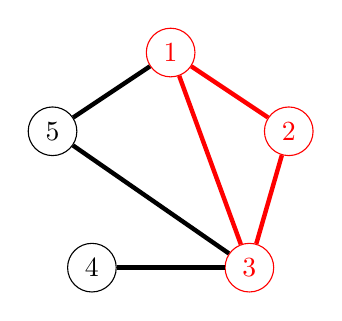
\begin{tikzpicture}[node distance={15mm}, main/.style = {draw, circle}] 
 \node[main][red] (1) at (1*90:1) {$1$};
 \node[main][red] (2) at (2*0:1.5) {$2$};
 \node[main] (5) at (3*60:1.5) {$5$};
 \node[main] (4) at (4*60:2) {$4$};
 \node[main][red] (3) at (5*60:2) {$3$};

\draw[ultra thick][red] (1) -- (2);
\draw[ultra thick][red] (2) -- (3);
\draw[ultra thick][red] (1) -- (3);
\draw[ultra thick][black] (1) -- (5);
\draw[ultra thick][black] (4) -- (3);
\draw[ultra thick][black] (5) -- (3);


    \end{tikzpicture}
    \caption{Graf $G$ wraz z zaznaczonym zbiorem niedozwolonym $S$}
    \label{SKlika}
 \end{figure}
 

 Zaaplikowanie własności 1 dla przedziału $P$ i pierwszego wierzchołka ze zbioru niedozwolonego czyli $\{1\}$ daje nam  
$$[\{5\},\{1,2,3,4,5\}] = [\{1,5\},\{1,2,3,4,5\}] \cup [\{5\},\{2,3,4,5\}]$$ 
Warto zauważyć, że drugi z wynikowych przedziałów nie łamie już ograniczenia narzuconego przez $P$, a więc można dodać go do listy przedziałów i kontynuować podział jedynie na pierwszym z przedziałów wynikowych. Analogiczna sytuacja zachodzi na każdym etapie podziału, ze względu na naturę ograniczenia wypływającego z kliki, gdzie usunięcie jednego z wierzchołków kliki powoduje akceptacje połączenia do reszty z nich. 

Kontynuujemy podział pozostałego przedziału dla kolejnego wierzchołka ze zbioru $\{2\}$
$$[\{1,5\},\{1,2,3,4,5\}] = [\{1,2,5\},\{1,2,3,4,5\}] \cup [\{1,5\},\{1,3,4,5\}]$$ 
Po raz kolejny można zaakceptować drugi z przedziałów i kontynuować podział pierwszego przez kolejny i ostatni wierzchołek $\{3\}$: 
$$[\{1,2,5\},\{1,2,3,4,5\}] = [\{1,2,3,5\},\{1,2,3,4,5\}] \cup [\{1,2,5\},\{1,2,4,5\}]$$
Po podziale przez ostatni z wierzchołków można, jak po każdym kroku, zaakceptować drugi z wynikowych przedziałów. Pierwszy z nich natomiast zawiera zbiór niedozwolony w stożku ograniczającym od dołu. Można go odrzucić ze względu na to, że wszystkie stożki takiego przedziału opisują niedozwolone rozszerzenia grafu $F$.

Podział przedziału dla zbioru niezależnego przeprowadzany jest w bardzo podobny sposób. Na każdym etapie podziału akceptowany jest pierwszy przedział wynikowy zamiast drugiego. W ramach przykładu podziału dla zbioru niezależnego załóżmy, że 
$P = [\emptyset,\{1,2\}]$ oraz $S = \{1,2,3,4\}$ i $S$ jest zbiorem niezależnym. Mamy również inny graf $G$, rysunek \ref{roszerzenieN}.
\begin{figure}[H]
  \centering
   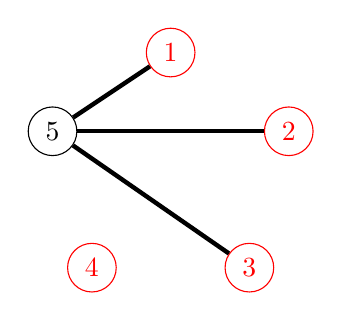
\begin{tikzpicture}[node distance={15mm}, main/.style = {draw, circle}] 
 \node[main][red] (1) at (1*90:1) {$1$};
 \node[main][red] (2) at (2*0:1.5) {$2$};
 \node[main] (5) at (3*60:1.5) {$5$};
 \node[main][red] (4) at (4*60:2) {$4$};
 \node[main][red] (3) at (5*60:2) {$3$};

\draw[ultra thick][black] (2) -- (5);
\draw[ultra thick][black] (1) -- (5);
\draw[ultra thick][black] (5) -- (3);

    \end{tikzpicture}
    \caption{Graf $G$ wraz z zaznaczonymi wierzchołkami należącymi do zbioru niedozwolonego $S$}
    \label{roszerzenieN}
 \end{figure}
 

W takim wypadku zbiór wierzchołków, wzdłuż którego dokonujemy podziału, nie obejmuje wszystkich wierzchołków należących do $S$. Jest tak dlatego, że część z nich należy już do $T_P$ i nie ma potrzeby ani możliwości dzielić przedziału przy ich pomocy. Dla pomniejszego zbioru wierzchołków $\{1,2\}$ pierwszym etapem podziału będzie 
$$[{\emptyset},\{1,2\}]= [\{1\},\{1,2\}] \cup [{\emptyset},\{2\}]$$ Akceptujemy pierwszy przedział i przechodzimy do kolejnego kroku
$$ [{\emptyset},\{2\}]= [\{2\},\{2\}] \cup [{\emptyset},{\emptyset}]$$ Po przejściu wszystkich wierzchołków i zaakceptowaniu pierwszego przedziału można odrzucić drugi, ponieważ wszystkie stożki przez niego objęte łamią ograniczenie narzucone przez $S$.


Rozumowanie dla ograniczenia wynikającego z kliki przebiega następująco:
\begin{algorithm}[H]
  \caption{Porównanie przedziału $P$ do zbioru niedozwolonego $S$ opisującego klikę}
  \begin{algorithmic}
  \IF{$S \subseteq T_P$}
	\IF{$S\subseteq B_P $} 
	  \STATE Usuń $P$ z listy przedziałów
	\ELSE
	  \STATE Podziel przedział $P$ wzdłuż $S \setminus B_P  $
  	\ENDIF
  \ENDIF  
  \end{algorithmic}
\end{algorithm}

Rozumowanie dla ograniczenia wynikającego ze zbioru niezależnego przebiega z kluczowymi różnicami w warunkach oraz sposobie podziału:

\begin{algorithm}[H]
  \caption{Porównanie przedziału $P$ do zbioru niedozwolonego $S$ opisującego zbiór niezależny}
  \begin{algorithmic}
  \IF{$S \not\subseteq B_P$}
	\IF{$S\not\subseteq T_P $} 
	  \STATE Usuń $P$ z listy przedziałów
	\ELSE
	  \STATE Podziel przedział $P$ wzdłuż $S \cap T_P  $
  	\ENDIF
  \ENDIF  
  \end{algorithmic}
\end{algorithm}

Warto zauważyć, że w przypadku podziału przedziałów w taki sposób mamy gwarancje, że jeżeli przedział $P$ spełnia ograniczenie, to wszystkie jego podprzedziały również je spełniają. Ze względu na to, po zaaplikowaniu wszystkich ograniczeń, pozostałe przedziały zawierają tylko takie połączenia, które spełniają wszystkie ograniczenia. Oznacza to, że te przedziały rozszerzenia grafu $F$ o wierzchołek tak, że nie jest zaburzona jego ramseyowskość.  
